\chapter{Reinforcement Learning Preliminaries}
This chapter is dedicated to present a concise theory of reinforcement learning. The first section will show how a certain goal can be formalized as a reward maximization -- one of the ideas which serves as a basic foundation of \acs{RL}. Section \ref{sec:mdp} explains the basics of \acs{MDP}, a general framework used in \acs{RL} problem. The notion of value function will be discussed in Section \ref{sec:value}. Subsequently, a method to solve \acs{RL}, namely policy and value iteration will be developed in section \ref{sec:value_iter}. Finally, Section \ref{sec:actor} will discuss the actor-critic structure which is an alternative solution to policy iteration.

\section{Goal as Cost Minimization}
The nature of \acs{RL} is inspired by the way living organisms learn to reach their desired goals. Animals for instance, learn by first acting on the environment, observe the changes that occur, and improve their action iteratively. One example is a circus lion that is tasked to perform acrobatic show while its trainer observing the progress. If the lion successfully executes the task, it will be rewarded with foods. Conversely, punishment will be inflicted whenever it fails. The lion initially has no idea of how to perform the task. However through trial and error, it will follow its instinct to increase the frequency of receiving rewards while trying its best to avoid punishments. In a certain duration of training, the circus lion will be finally able to perform the task flawlessly. 

Now we will formalize above illustration for robotics application. A robot can be described by its states $x_k$ with subscript $k$ denoting time instance. Applying an action $u_k$ will bring the robot to state $x_{k+1}$ with immediate reward $r_{k+1}$. Subsequently, at $k+1$ the robot applies $u_{k+1}$ which yields state $x_{k+2}$ and $r_{k+2}$. This action-state-update iteration is run for infinite time instances. The goal is defined as maximization of cumulative reward the robot receives. In control engineering, reward is usually replaced with cost. In that case the goal is defined as minimization problem. Starting from now, we will define goal as minimization of future cost $J$.

From the sequence of cost obtained over time, we can define a formalization of goal, called expected return. Return $J_t$ is a function that maps the sequence of costs into real number. An example of return is the sum of the costs:

\begin{equation}
J_t = r_{t+1} + r_{t+2} + r_{t+3} + \dots + r_T
\end{equation} 

\section{Markov Decision Process} \label{sec:mdp}
\ac{MDP} is defined as a tuple $\left<X, U, f, \rho \right>$ which satisfies Markov property \cite{babuskaRL}. The detailed explanation of Markov property can be found on \cite{sutton1998reinforcement} section 3.5 but the main idea is that to determine the probability of a state at certain time, it is sufficient to only know the state of previous time instance. The elements of the tuple are:
\begin{itemize}
	\item $X$ is the state space
	\item $U$ is the action space
	\item $f :X \times U \rightarrow X$ is the state transition function (system dynamics) 
	\item $\rho:X \times U \rightarrow \mathbb{R}$ is the reward function
\end{itemize}

In control engineering, $f$ represents the system dynamics which is a transition function mapping a current state and action to the one-step ahead state up to a probability distribution. This probability distribution is mathematically denoted as

\begin{equation}
	\text{Pr}\{x_{t+1} = x', r_{t+1} = r| x_t, u_t \}
	\label{eq:markov}
\end{equation}
where $x$ denotes state, $u$ denotes action, and $r$ denotes immediate reward obtained upon applying the input on the corresponding state. 



\section{Value Function} \label{sec:value}
Value function describes how good a particular state or state-action pair under a certain policy. As previously explained, in this thesis we will stick to control engineering convention by seeing \acs{RL} as cost minimization problem. Therefore, the smaller value function of a state $x$, the better it is. The value function is denoted by $ V^{\pi}(x) $ for state-value function and $ Q^{\pi}(x,u) $ for action-value function under policy $\pi$. It can be written in terms of immediate reward and the value function of the next state by following derivation
\begin{equation}
\begin{split}
V^{\pi}(x_t) &= \rho(x_t,u_t) + \gamma \rho(x_{t+1},u_{t+1}) + \gamma^2 \rho(x_{t+2},u_{t+2}) + ... + \gamma^{\infty}\rho(x_{\infty},u_{\infty}) \\
V^{\pi}(x_t) &= \rho(x_t,u_t) + \gamma \left( \rho(x_{t+1},u_{t+1}) + \gamma^2 \rho(x_{t+2},u_{t+2}) + ... + \gamma^{\infty}\rho(x_{\infty},u_{\infty})\right)  \\
V^{\pi}(x_t) &= \rho(x_t,u_t) + \gamma V^{\pi}(x_{t+1})
\end{split}
\end{equation} 

Furthermore, one can always find a policy which gives an optimal value function $V^*$. This optimal value function respects the Bellman optimality equation, which can be written as 
\begin{equation}
V^*(x_t) = \rho(x,u) + \gamma \min_{u} V^*(x_{t+1})
\label{eq:bellman}
\end{equation}
Similarly, the action-value function is

\begin{equation}
Q^*(x_t,u_t) = \rho(x,u) + \gamma \min_{u} Q^*(x_{t+1},u_{t+1})
\label{eq:bellman2}
\end{equation}

Discount factor $\gamma$ is introduced to avoid the value function goes to infinity. Once $V^*$ is known, the optimal policy can be taken in a greedy way as
\begin{equation}
\pi^* = \text{arg} \max_{\pi} V^*(x)
\label{eq:optPi}
\end{equation}
This concludes the formulation of \acs{RL} problem. The subsequent sections will deal with two methods to solve for the solution.

\section{Policy and value iteration} \label{sec:value_iter}
\ac {PI} and \ac{VI} belong to a class of elementary solution to the \acs{RL} called  dynamic programming \cite{sutton1998reinforcement}. They are characterized by the requirement of system model $f$. These methods are closely related with a branch of control system, namely optimal control \cite{126844}.

\acs {PI} is a two steps algorithm, consists of policy evaluation and policy improvement. Let the initial policy at certain state $x$ be given by $ \pi$. A better policy can be determined by first evaluating the old policy's value $ V^{\pi} $, search for the optimal action at state $x$ greedily, and replace the old policy with the optimal action. This process can be casted as Algorithm~\ref{alg:PI}. Note that the policy evaluation step is actually a Bellman equation \eqref{eq:bellman} turned into assignment. The \textit{policy-stable} variable is to indicate that the policy does not change anymore i.e. converged.

\begin{algorithm}
	\textbf{Initialization:} \\
	Start from an admissible policy $ \pi $\\
	Initialize $V^{\pi}(x)$ arbitrarily, e.g. $ V^{\pi}(x) = 0 \hspace{2mm}  \forall x \in \mathcal{X} $ \\
	\Repeat(){\textit{policy-stable} = true}{	
	\textbf{Policy Evaluation:} \\
		\Repeat(){$ \Delta  <  \varepsilon $ (a small positive number)}{
		$ \Delta $ $ \leftarrow $ 0 \\
		\textbf{For each} $ x \in \mathcal{X} $ :\\
			\hspace{5mm} $ v $ $ \leftarrow $ $ V^{\pi}(x) $ \\
			\hspace{5mm} $ V^{\pi}(x) \leftarrow \rho(x, \pi(x)) +\gamma V^{\pi}(x') $ \\
			\hspace{5mm} $ \Delta = $ max$ (\Delta, |v-V^{\pi}(x)|) $ \\}
			\vspace{2mm}
	\textbf{Policy Improvement:} \\
		\textit{policy-stable} $ \leftarrow $ false \\
		\textbf{For each} $ x \in \mathcal{X} $ : \\
			\hspace{5mm} $ b \leftarrow \pi(x) $ \\
			\hspace{5mm} $ \pi(x)=$  arg $\underset{u}{\text{min}} \hspace{1mm} \rho(x, u) +\gamma V^{\pi}(x') $  \\
			\hspace{5mm} \textbf{if} $ b = \pi(x) $ \textbf{then} \\ 
			\hspace{10mm} \textit{policy-stable} $ \leftarrow $ true \\
			\hspace{5mm} \textbf{endif}
	}
\caption{Policy iteration algorithm}
\label{alg:PI}
\end{algorithm}

\acs{VI} is similar to, but more efficient version than \acs{PI}. In order to increase computational efficiency, instead of evaluating value function $V$ for all possible state $x$ in every iteration, one can evaluate the value function in greedy way, which results in less iteration. Once the value function converges to $V^*$, the optimal policy can be directly obtained as the control input which minimizes $V$. This algorithm is shown in Algorithm~\ref{alg:VI}. 

\begin{algorithm}
	\textbf{Initialization:} \\
	Start from an admissible policy $ \pi $\\
	Initialize $V^{\pi}(x)$ arbitrarily, e.g. $ V^{\pi}(x) = 0 \hspace{2mm}  \forall x \in \mathcal{X} $ \\
	\Repeat(){policy converges to $ \pi^* $}{
		\Repeat(){$ \Delta  <  \varepsilon $ (a small positive number)}{
			$ \Delta $ $ \leftarrow $ 0 \\
			\textbf{For each} $ x \in \mathcal{X} $ :\\
			\hspace{5mm} $ v $ $ \leftarrow $ $ V^{\pi}(x) $ \\
			\hspace{5mm} $ V^{\pi}(x) \leftarrow \underset{u}{\text{min}} \rho(x, \pi(x)) + \gamma V^{\pi}(x') $ \\
			\hspace{5mm} $ \Delta = $ max$ (\Delta, |v-V^{\pi}(x)|) $ \\}
		\vspace{2mm}
		Obtain a deterministic policy: \\
		$ \pi(x)=$  arg $\underset{u}{\text{min}} \hspace{1mm} \rho(x, u) +\gamma V^{\pi}(x') $  \\

	}
	\caption{Value iteration algorithm}
\label{alg:VI}
\end{algorithm}

 
\section{Actor Critic Method} \label{sec:actor}
The second method for solving \acs{RL} is by using temporal-difference learning. It is favored due to its model-free nature. In this section, we will discuss a class of \ac{TD} called actor-critic method. The idea of actor-critic method is to separate policy and value function into entities called actor and critic respectively (see Figure~\ref{fig:actorCritic}). The critic evaluates and criticizes the actor performance by feeding a temporal difference signal $\delta$ to the actor. This signal is basically the difference between right and left hand side of Bellman equation, in other words, the Bellman equation error. 

In order to deal with continuous state space, the actor $\psi$ and critic $\theta$ functions are parameterized by function approximators. Examples of function approximators are fuzzy, neural networks and tile coding. The actor-critic method is presented in Algorithm~\ref{alg:actorcritic} (adapted from \cite{babuskaRL}). Note that $\tilde{u}$ denotes random exploration term which is needed to avoid getting stuck at local optimum.

%\begin{figure}[h!]
%\centering
%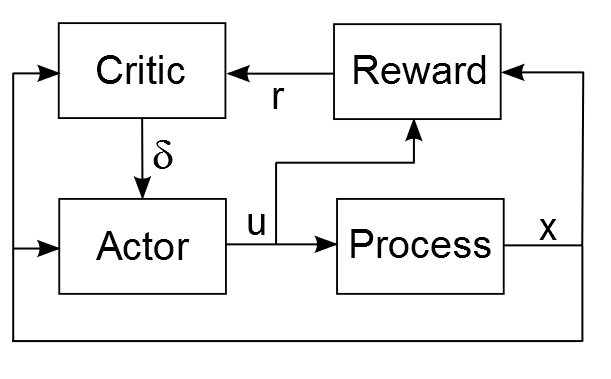
\includegraphics[width=0.6\linewidth]{actorCritic2}
%\caption{Actor critic structure (diagram reproduced from \cite{babuskaRL})} 
%\label{fig:actorCritic}
%\end{figure}
\tikzstyle{block} = [draw, fill=blue!20, rectangle, 
minimum height=3em, minimum width=6em]
\tikzstyle{sum} = [draw, fill=blue!20, circle, node distance=1cm]
\tikzstyle{input} = [coordinate]
\tikzstyle{output} = [coordinate]
\tikzstyle{pinstyle} = [pin edge={to-,thin,black}]


\begin{figure}
	\centering
	\begin{tikzpicture}[auto, node distance=2cm,>=latex' ]
	\node [block] (critic) {Critic};
	\node [block, right of=critic, node distance=4cm] (reward) {Reward};
	
	\draw[decoration={markings,mark=at position 1 with {\arrow[ultra thick]{>}}},
	postaction={decorate}] (reward) -- node[name=r] {$r$} (critic);	
	
	\node [output, right of=reward] (output) {};
	\node [block, below of=reward] (process) {Process};
	\node [block, below of=critic] (actor) {Actor};
	
	\draw[decoration={markings,mark=at position 1 with {\arrow[ultra thick]{>}}},
	postaction={decorate}] (process.east)  -- ++(1,0) |- node[pos=0.1] {$x$}  (reward.east);
	
	\draw[decoration={markings,mark=at position 1 with {\arrow[ultra thick]{>}}},
	postaction={decorate}] (process.east)  -- ++(1,0) -- ++(0,-1) -- ++(-8,0)  |- node[pos=0.1] {}  (actor.west);
	
	\draw[decoration={markings,mark=at position 1 with {\arrow[ultra thick]{>}}},
	postaction={decorate}] (process.east)  -- ++(1,0) -- ++(0,-1) -- ++(-8,0)  |- node[pos=0.1] {}  (critic.west);	
	
	\draw[decoration={markings,mark=at position 1 with {\arrow[ultra thick]{>}}},
	postaction={decorate}] (actor) -- node[pos=0.20] {$u$} (process);	
	
	\draw[decoration={markings,mark=at position 1 with {\arrow[ultra thick]{>}}},
	postaction={decorate}] (actor.east)  -- ++(0.8,0) -- ++(0,1) -- ++(2,0) -- ++(0,0.44) node[pos=0.1] {}  (reward.south);	
	
	\draw[decoration={markings,mark=at position 1 with {\arrow[ultra thick]{>}}},
	postaction={decorate}] (critic.south)  --  node[] {$\delta$}  (actor.north);		

	\end{tikzpicture}
\caption{Actor critic structure (diagram reproduced from \cite{babuskaRL})} 
\label{fig:actorCritic}
\end{figure}

	

\begin{algorithm}
	\For{every trial}{
		Initialize $x_0$ and $u_0 = \tilde{u}_0$\\
		\Repeat{terminal state}{
			apply $u_k$, measure $x_{k+1}$, receive $r_{k+1}$ \\
			choose next action $ u_{k+1} = \hat{\pi}(x_{k+1}, \psi_k)	+ \tilde{u}_{k+1} $ \\
			$ \delta_k = r_{k+1} + \hat{V}(x_{k+1}, \theta_k) - \hat{V}(x_{k}, \theta_k) $ \\
			$ \theta_{k+1} = \theta_k + \alpha_c\delta_k \frac{\partial \hat{V}(x,\theta)}{\partial \theta} \bigg|_{x=x_k, \theta = \theta_k}$ \\
			$ \psi_{k+1} = \psi_k + \alpha_c\delta_k \frac{\partial \hat{V}(x,\psi)}{\partial \psi} \bigg|_{x=x_k, \psi = \psi_k}$
		}
	}
	\caption{Actor-critic algorithm}
	\label{alg:actorcritic}
\end{algorithm}


